\chapter{ideal Bose systems}
\begin{itemize}
	\item 根据 \eqref{5.4.2}, 如果 $n \lambda^3 \ll 1$ 的条件不再满足, 就需要考虑量子效应.
	\begin{itemize}
		\item 需要分别讨论可以对 $n \lambda^3 \lesssim 1$ 作级数展开的区间, 和 $n \lambda^3 \gtrsim 1$ 系统完全偏离经典统计的情况.
	\end{itemize}
	
	\item $g_n(z)$ 是 Bose-Einstein function,
	\begin{equation}
		g_n(z) = z + \frac{z^2}{2^n} + \frac{z^3}{3^n} + \cdots
	\end{equation}
	是单调递增函数, 且 $g_n(1) = \zeta(n)$.
\end{itemize}

\section{thermodynamics behavior of an ideal Bose gas}
\begin{itemize}
	\item ideal Bose gas 的 grand partition function 为
	\begin{equation} \label{7.1.1}
		\frac{P V}{k_B T} = \ln Z_\text{GC} = N_s \Big( \frac{V}{\lambda^3} g_{5 / 2}(z) - \underbrace{\ln(1 - z)}_{\text{negligible}} \Big),
	\end{equation}
	其中 $z = e^{\beta \mu} < 1$ 是 fugacity (见 \eqref{1.3.3}), $N_s$ 是粒子的自旋状态数.
	
	\begin{tcolorbox}[title=calculation:]
		注意到粒子能量 $\epsilon$ 的简并度为 (根据 \eqref{1.2.3})
		\begin{equation}
			g(\epsilon) = N_s 2 \pi \frac{V / \lambda^3}{(\pi k_B T)^{3 / 2}} \epsilon^{1 / 2},
		\end{equation}
		所以 (另外 $g_0 = N_s \neq 0$, 而 $g(0) = 0$, 需要把 $\epsilon = 0$ 单独拿出来)
		\begin{align}
			\ln Z_\text{GC} &= - N_s \ln(1 - z) - N_s 2 \pi \frac{V / \lambda^3}{(\pi k_B T)^{3 / 2}} \int_0^\infty \ln(1 - z e^{- \beta \epsilon}) \epsilon^{1 / 2} d\epsilon \notag \\
			&= - N_s \ln(1 - z) - N_s \frac{2 \pi}{\pi^{3 / 2}} \frac{V}{\lambda^3} \int_0^\infty \ln(1 - z e^{- x}) x^{1 / 2} dx = \cdots
		\end{align}
		注意 $\ln(1 - z)$ 在 $z = 1$ 处有一个极点, 所以 Taylor 展开收敛的条件是
		\begin{equation} \label{7.1.4}
			z e^{- x} < 1 \Longrightarrow z < 1.
		\end{equation}
	\end{tcolorbox}
	
	\begin{itemize}
		\item 基态上的粒子数 $N_0$ 可以忽略.
		
		\begin{tcolorbox}[title=proof:]
			注意到
			\begin{equation}
				N_0 = N_s \frac{1}{z^{- 1} - 1} \Longrightarrow z = \frac{N_0 / N_s}{N_0 / N_s + 1},
			\end{equation}
			那么 grand partition function \eqref{7.1.1} 中基态贡献的项为
			\begin{equation}
				- N_s \ln(1 - z) = N_s \ln(N_0 / N_s + 1) < O(\ln N),
			\end{equation}
			而 $\ln Z_\text{GC} \sim N$, 因此可以忽略.
		\end{tcolorbox}
	\end{itemize}
	
	\item 得到
	\begin{equation}
		\begin{dcases}
			N = N_s \frac{V}{\lambda^3} g_{3 / 2}(z) + N_s \frac{1}{z^{- 1} - 1} \\
			U = \frac{3 N_s}{2} k_B T \frac{V}{\lambda^3} g_{5 / 2}(z)
		\end{dcases},
	\end{equation}
	和 equation of state (in the form of virial expansion, 见 \eqref{3.5.12}),
	\begin{equation}
		\frac{P V}{N k_B T} = \begin{dcases}
			\frac{g_{5 / 2}(z)}{g_{3 / 2}(z)} = \sum_{l = 1}^\infty a_l (n \lambda^3 / N_s)^{l - 1} & T \gg T_c, \ \text{virial expansion} \\
			\frac{1}{n \lambda^3 / N_s} \zeta({\textstyle \frac{5}{2}}) & T < T_c
		\end{dcases},
	\end{equation}
	($T \gg T_c$ 指要求级数收敛), 其中 virial coefficients are
	\begin{align}
		& a_1 = 1, \quad a_2 = - \frac{1}{4 \sqrt{2}} \approx - 0.177, \quad a_3 = - \Big( \frac{2}{9 \sqrt{3}} - \frac{1}{8} \Big) \approx - 0.0033, \notag \\
		& a_4 = - \Big( \frac{3}{32} + \frac{5}{32 \sqrt{2}} - \frac{1}{2 \sqrt{6}} \Big) \approx - 0.00011.
	\end{align}
	
	\item 注意到 $U = \frac{3}{2} P V$, 系统的 specific heat 为
	\begin{equation}
		\frac{C_V}{N k_B} = \begin{dcases}
			\frac{3}{2} \sum_{l = 1}^\infty \frac{5 - 3 l}{2} a_l (n \lambda^3 / N_s)^{l - 1} & T \gg T_c \\
			\frac{15}{4} \frac{\zeta({\textstyle \frac{5}{2}})}{\zeta({\textstyle \frac{3}{2}})} \Big( \frac{T}{T_c} \Big)^{\frac{3}{2}} & T < T_c
		\end{dcases}.
	\end{equation}
	
	\item 得到 $T$-$P V$ 和 $T$-$C_V$ 曲线, 如下图:
	
	\begin{figure}[H]
		\centering
		\begin{subfigure}{0.4\linewidth}
			\centering
			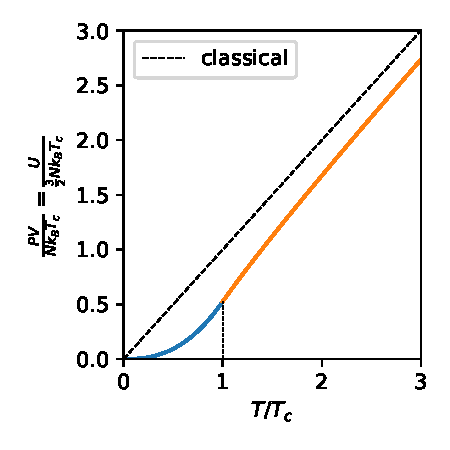
\includegraphics[scale=0.8]{figures/plot of T-PV.pdf}
			\caption{plot of $T$-$P V$.}
		\end{subfigure}
		\begin{subfigure}{0.4\linewidth}
			\centering
			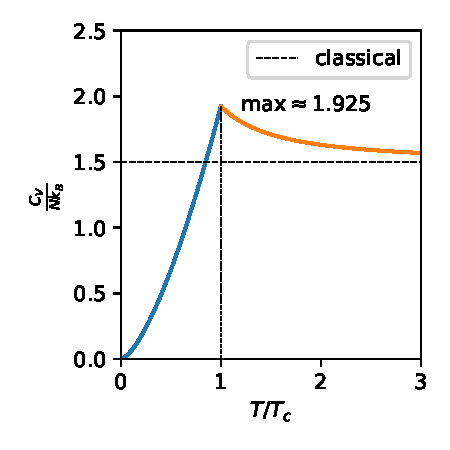
\includegraphics[scale=0.8]{figures/plot of T-C_V.pdf}
			\caption{plot of $T$-$C_V$.}
		\end{subfigure}
		\caption{}
	\end{figure}
	
	可见 $T = T_c$ 时存在相变.
\end{itemize}

\subsection{normal phase and condensed phase}
\begin{itemize}
	\item grand partition function 计算方法的前提条件是 \eqref{7.1.4}, (代入 $N$-$z$ 关系式) 等价于
	\begin{equation}
		N_e < N_s \frac{V}{\lambda^3} \underbrace{\zeta({\textstyle \frac{3}{2}})}_{\approx 2.612},
	\end{equation} 
	其中 $N_e$ 表示激发态上的粒子数量.
	
	\item 当 $z$ 接近 $1$ 时, $N_0 = N_s \frac{1}{z^{- 1} - 1} \gg 1$, 此时,
	\begin{equation}
		\begin{dcases}
			z = 1 - \frac{N_s}{N_0} \\
			N_0 = N - N_s \frac{V}{\lambda^3} \zeta({\textstyle \frac{3}{2}}) \gg 1
		\end{dcases},
	\end{equation}
	几乎所有粒子都处于基态, 称为 Bose-Einstein condensation.
	
	\item 发生 Bose-Einstein condensation 的条件是 $N > N_s \frac{V}{\lambda^3} \zeta(\frac{3}{2})$, 或者
	\begin{equation}
		n \lambda^3 / N_s > \zeta({\textstyle \frac{3}{2}}) \iff T < T_c = \frac{h^2}{2 \pi m k_B} \Big( \frac{N / N_s}{V \zeta(\frac{3}{2})} \Big)^{\frac{2}{3}},
	\end{equation}
	此时, 系统可以认为处于两相混合态: 由 $N_e$ 个处于激发态的粒子 (in the normal phase), 和 $N_0$ 个处于基态的粒子 (in the condensed phase) 组成.
	\begin{itemize}
		\item 一个对化简有用的公式,
		\begin{equation}
			\frac{T}{T_c} = \Big( \frac{\zeta({\textstyle \frac{3}{2}})}{n \lambda^3 / N_s} \Big)^{\frac{2}{3}}.
		\end{equation}
		
		\item $T < T_c$ 时,
		\begin{equation}
			\frac{N_0}{N} = 1 - \Big( \frac{T}{T_c} \Big)^{\frac{3}{2}} \overset{T = T_c - 0^+}{\approx} \frac{3}{2} \frac{T_c - T}{T_c}.
		\end{equation}
	\end{itemize}
	
	\item 综上, $z$ 随 $T$ 变化曲线如下图:
	
	\begin{figure}[H]
		\centering
		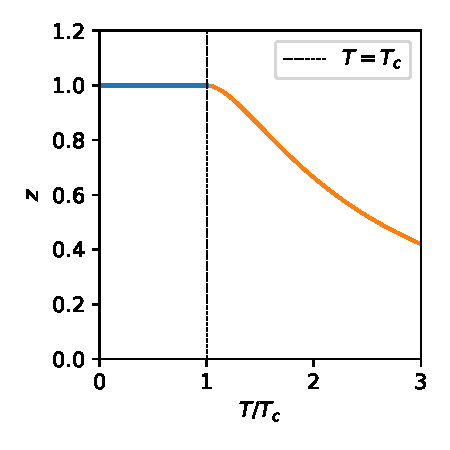
\includegraphics[scale=0.8]{figures/plot of T-z.pdf}
		\caption{plot of $T$-$z$.}
	\end{figure}
\end{itemize}
